\begin{frame}[t]{TS912 - Recherche} 

    Eine einfache Recherche für uns zu einem Hersteller, hier zum Beispiel ST.
    \href{https://www.st.com/en/amplifiers-and-comparators/ts912.html}{https://www.st.com/en/amplifiers-and-comparators/ts912.html}


    \begin{spacing}{0.9} \begin{tiny}
        \begin{table}[h!]
          \begin{tabular}{p{5cm} p{5cm}}
              \begin{minipage}{0.5\textwidth}
                  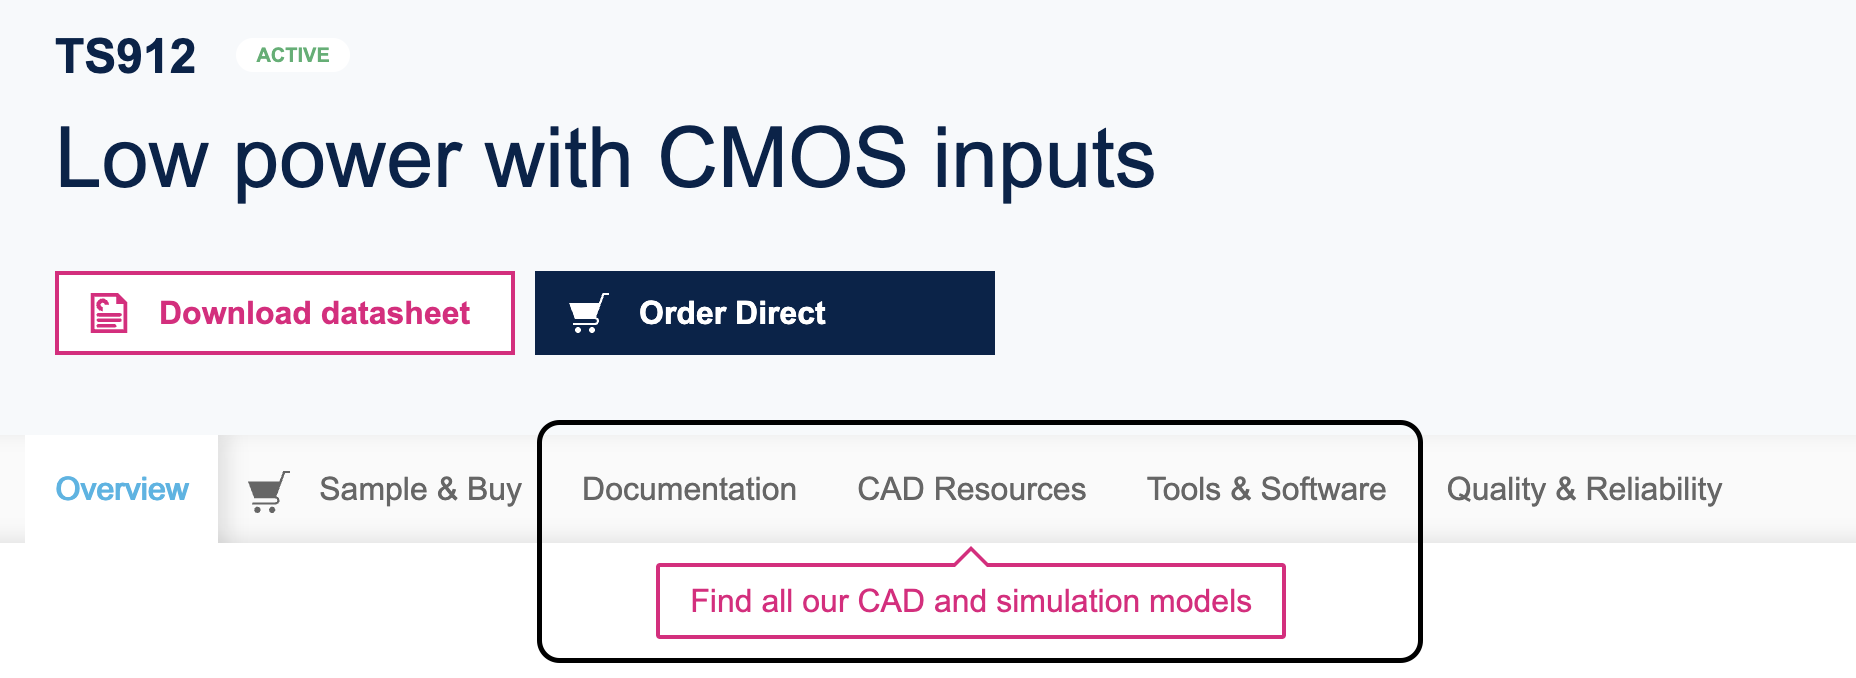
\includegraphics[width=\linewidth]{pictures/spice_model_search.png}
              \end{minipage} 
              &
              \begin{minipage}{0.5\textwidth}
                  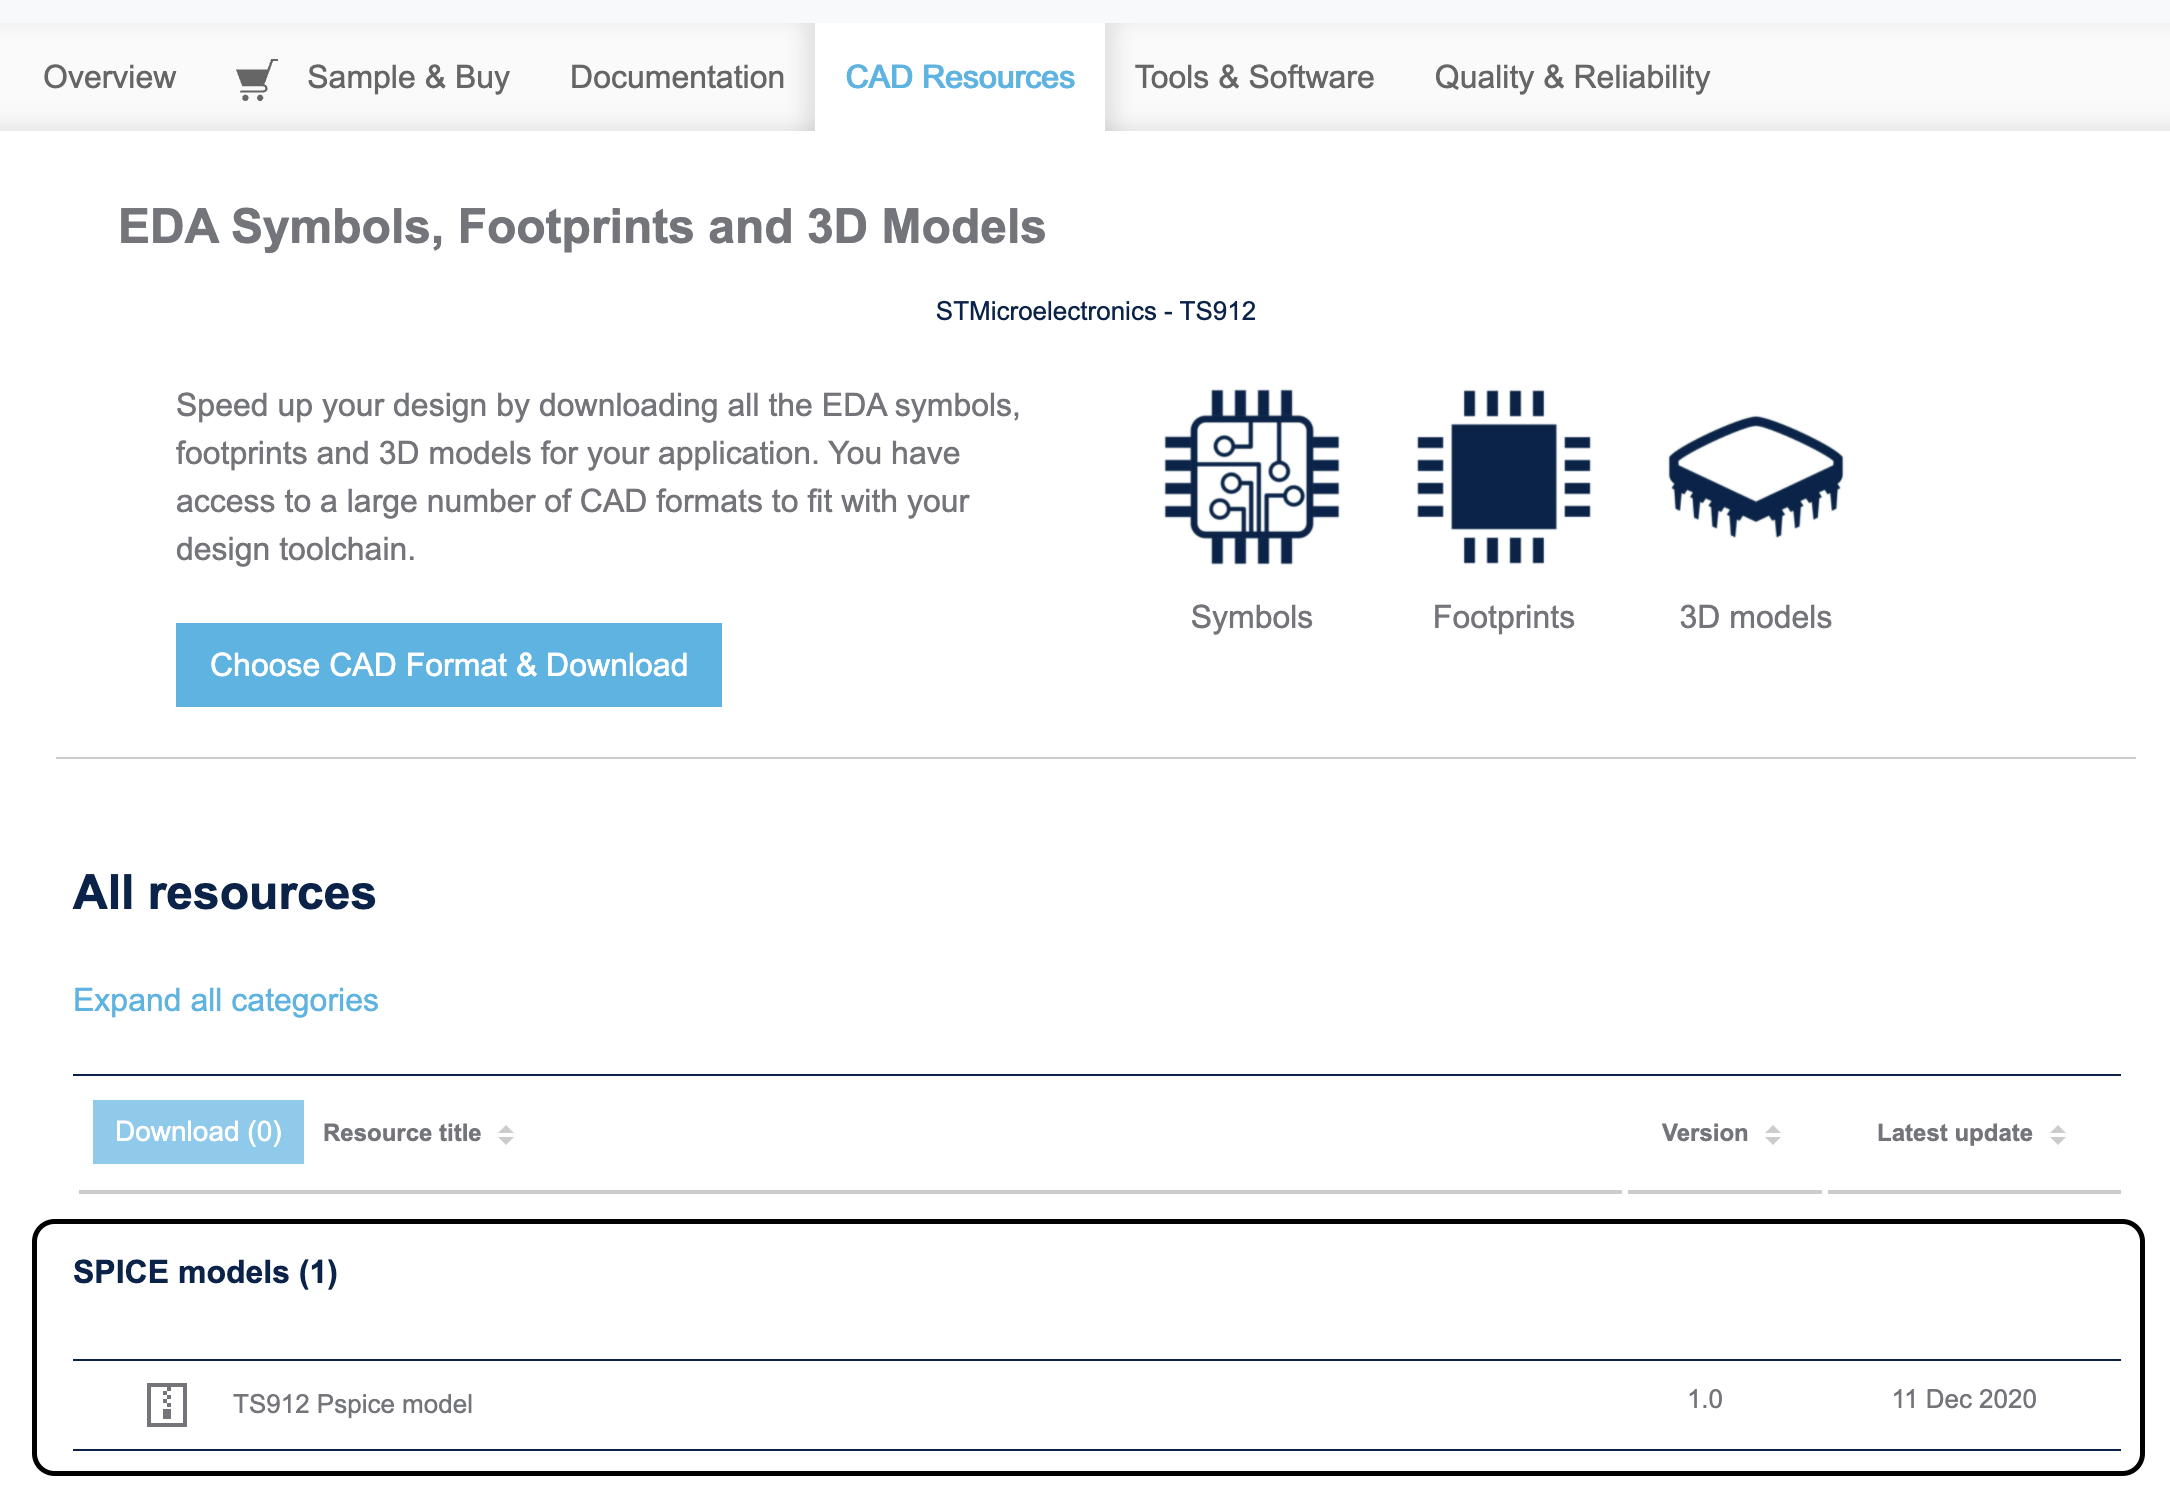
\includegraphics[width=\linewidth]{pictures/spice_model_search2.png}
              \end{minipage} 
        \end{tabular}
      \end{table}
      \end{tiny} \end{spacing}

\end{frame}

\begin{frame}[t]{Subscircuit erstellen} 

    Ein spice Model ist eine einfache Text-Datei, die einfach in LTSpice eingebunden werden kann.
    Kopiert den \textbf{subcircuit} dazu in eine Text-Datei mit der Endung .sub \textbf{ts912.sub} und speichert diese im Ordner:

    \begin{scriptsize}
        \begin{enumerate}
            \item Windows \textbf{LTSpice / lib / sub} 
            \item MacOS \textbf{/Users/"user"/Library/ApplicationSupport/LTspice/lib/sub}.
        \end{enumerate}
    \end{scriptsize}

    \begin{spacing}{0.9} \begin{tiny}
        \begin{minipage}{\textwidth}
          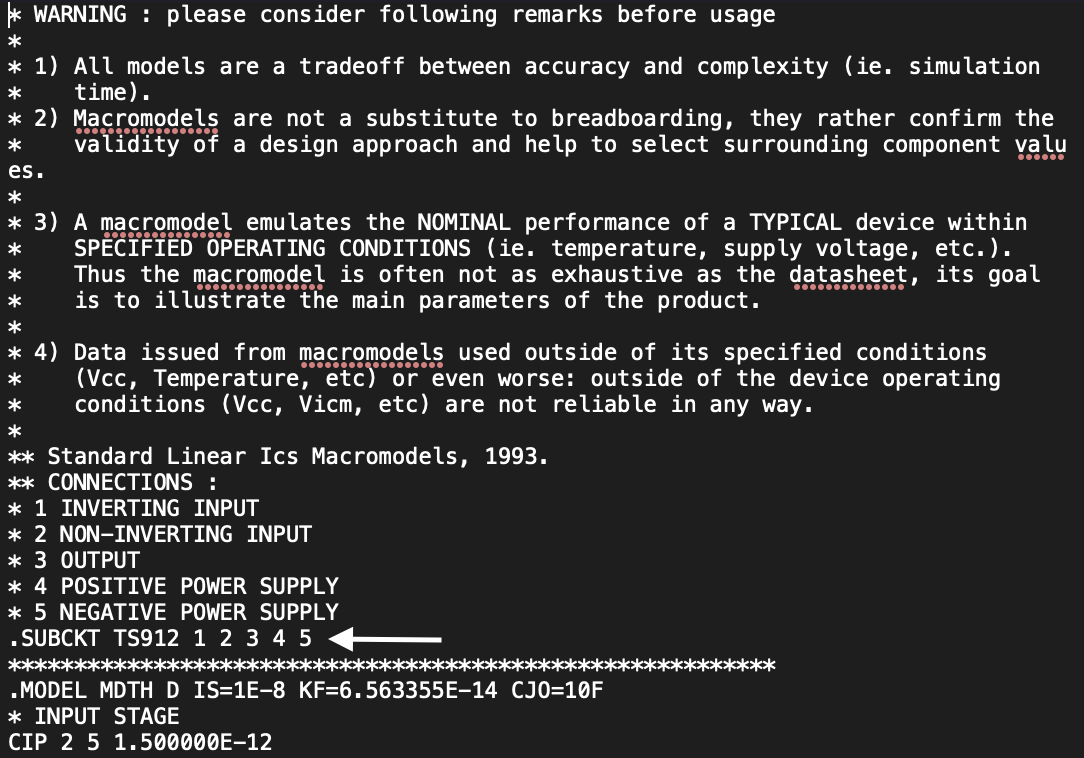
\includegraphics[width=0.5\linewidth]{pictures/spice_model.png}
        \end{minipage}
    \end{tiny} \end{spacing}
\end{frame}

\begin{frame}[t]{LTSpice Symbol erstellen} 

    ...
\end{frame}

\begin{frame}[t]{Bauteil verwenden} 

    ...
\end{frame}